\chapter{Integración de ROS en OpenROV}
\label{cap:integracionROS}

En este capítulo se va a describir cómo se ha realizado la integración de ROS con OpenROV\cite{ros_rov}.

Para ello, utilizaremos las bibliotecas de ROS Rosbridge y Roslibjs, que nos proporcionarán la comunicación entre el ordenador y el robot OpenROV.

\section{Configuración del ROV}
\label{cap:Configuracion del ROV}
La electrónica de OpenROV se basa en un Arduino conectado a una placa BeagleBone, que ejecutará el software de OpenROV.

Para la implementación de ROS con OpenROV se ha decidido instalar ROS en el portátil en lugar de en el ROV, ya que se necesita ejecutar un ROS Master. Si se hubiera realizado a la inversa, se necesitaría acceso al robot para ejecutar el ROS Master, por lo que una vez sumergido no podríamos utilizar ROS.

El ROS Master se ejecutará en el portátil y será el que interactúe con los nodos de ROS instalados, en este caso, Rosbridge.

Para la comunicación de ROS y OpenROV usaremos el paquete Roslibjs, el cual instalaremos dentro del software del robot. Roslibjs es la biblioteca que utiliza JavaScript para comunicarse con ROS. Roslibjs publicará y/o suscribirá a los mensajes de ROS.

Se utilizará el paquete de Rosbridge para traducir los mensajes JSON en mensajes ROS (OpenROV utiliza JSON para su comunicación). Este paquete actúa como un Nodo de ROS que puede publicar y/o suscribir a los mensajes.

En conclusión, la comunicación se realizará a través de una conexión Websocket (Rosbridge) y el paquete de Roslibjs.

La figura a continuación muestra la estructura básica de ROS para la integración de OpenROV.

\begin{figure} [hbtp]
  \begin{center}
    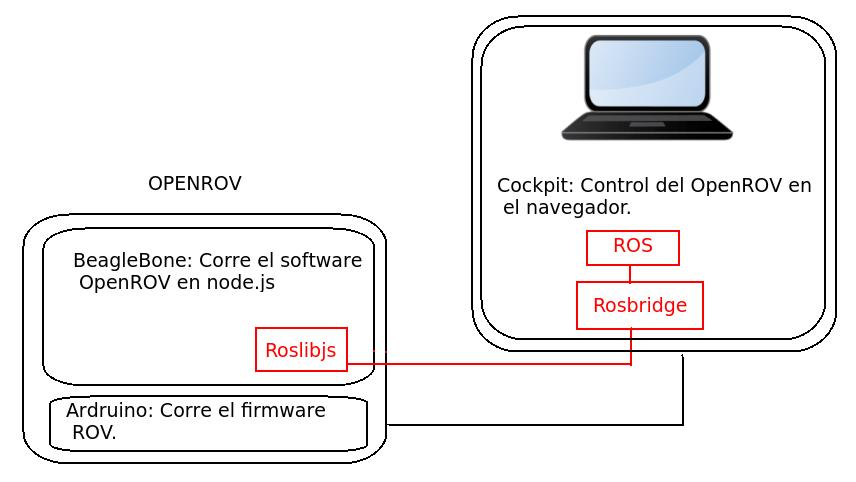
\includegraphics[width=8cm]{img/cap4/conect_ros_rov}
  \end{center}
  \caption{Diagrama de la conexión ROS y OpenROV}
  \label{fig:conect_ros_rov}
\end{figure}

Para configurar el robot se debe instalar el Roslibjs. Sin embargo, este paquete necesita de varias dependencias.

Comenzaremos configurando el BeagleBone a través de una conexión SSH, conectando un cable Ethernet entre el BeagleBone y el router.
Para activar el hardware usaremos un cable miniUSB conectado entre el BeagleBone y el portátil.
Una vez realizadas las conexiones, haremos un SSH a la placa.
\renewcommand{\lstlistingname}{}
\begin{lstlisting}[caption=SSH, label={lst:ssh}]
$ ssh rov@192.168.7.2
\end{lstlisting}
Cuando pida la contraseña, deberemos introducir “OpenROV”.

\begin{figure} [hbtp]
  \begin{center}
    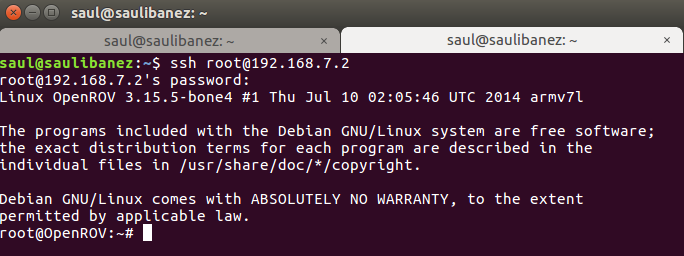
\includegraphics[width=12cm]{img/cap4/ssh}
  \end{center}
  \caption{SSH}
  \label{fig:ssh}
\end{figure}

Para instalar las dependencias de Roslibjs, ejecutaremos los siguientes comandos:

\renewcommand{\lstlistingname}{}
\begin{lstlisting}[caption=Dependencias Roslibjs, label={lst:roslibjs}]
sudo apt-get update 
sudo apt-get install libcairo2-dev libjpeg-dev libpango1.0-dev libgif-dev build-essential g++
\end{lstlisting}

\begin{figure} [hbtp]
  \begin{center}
    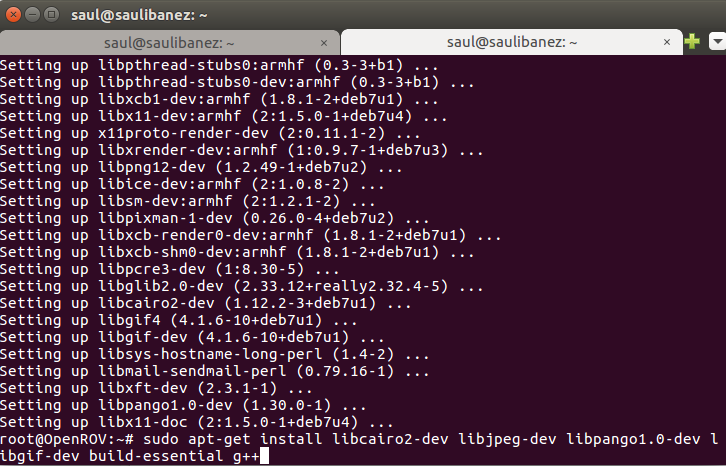
\includegraphics[width=12cm]{img/cap4/dependencias_roslibjs}
  \end{center}
  \caption{Dependencias Roslibjs}
  \label{fig:Dependencias Roslibjs}
\end{figure}
\newpage
Continuaremos instalando otras dependencias de Roslibjs. En este caso, npm, que es un gestor de paquetes que utiliza Node.js.
\\Para que no surjan errores con el proxy, debemos deshabilitarlo y realizar un reseteo del sistema. 
\renewcommand{\lstlistingname}{}
\begin{lstlisting}[caption=Dependencias Roslibjs, label={lst:roslibjs}]
$ sudo /etc/init.d/openrov-proxy stop
$ sudo /etc/init.d/openrov restart
$ sudo chown -R $USER /usr/local 
$ npm install canvas 
\end{lstlisting}

\newpage
\begin{figure} [hbtp]
  \begin{center}
    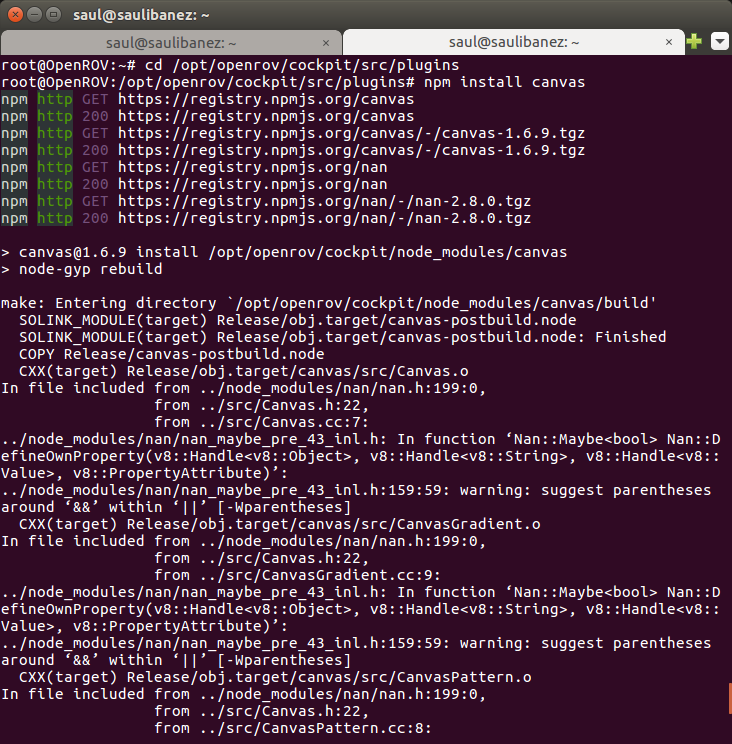
\includegraphics[width=12cm]{img/cap4/canvas}
  \end{center}
  \caption{Canvas}
  \label{fig:canvas}
\end{figure}

La última dependencia es Roslibjs, que lo instalaremos usando el siguiente comando: 
\renewcommand{\lstlistingname}{}
\begin{lstlisting}[caption=Roslib, label={lst:roslib}]
$ npm install roslib
\end{lstlisting}

Dentro de la carpeta /opt/openrov/cockpit/src/plugins, crearemos un directorio llamado ros (sudo mkdir ros) y en él, se creará un fichero llamado index.js, que ejecutará la conexión con el ROS Master localizado en el portátil.
\newpage
\renewcommand{\lstlistingname}{}
\begin{lstlisting}[caption=Conexión con ROS, label={lst:conection_ros}]
function ros(name, deps) {
  		console.log("ROS plugin started");

  		// Comienza la sesion de ROS
 		var ROSLIB = require("roslib")
  		var ros = new ROSLIB.Ros({
    			url : 'ws://192.168.7.1:9090'
  		});

  		ros.on('connection', function() {
   			console.log('ROS connected to websocket');
  		});

  		ros.on('error', function(error) {
    			console.log('ROS error connecting to websocket');
  		});

 		 ros.on('close', function() {
    			console.log('ROS closed websocket connection');
 		});
	};

	module.exports = ros;
\end{lstlisting}

También se debe modificar el fichero hosts (sudo vim /etc/hosts) y en él realizaremos los siguientes cambios:

\begin{lstlisting}[caption=/etc/hosts, label={lst:hosts}]
#127.0.1.1	OpenROV
192.168.7.2	OpenROV
192.168.7.1	saul.ibanez.local
\end{lstlisting}

\section{Configuración de ROS}
\label{cap:Configuracion de ROS}
Para la conexión con ROS, se decide instalar ROS Kinetic en el portátil:

\begin{lstlisting}[caption=Instalacion de ROS, label={lst:install_ros}]
sudo sh -c 'echo "deb http://packages.ros.org/ros/ubuntu $(lsb_release -sc) main" > /etc/apt/sources.list.d/ros-latest.list'
sudo apt-key adv --keyserver hkp://ha.pool.sks-keyservers.net:80 --recv-key 421C365BD9FF1F717815A3895523BAEEB01FA116
sudo apt-get update
sudo apt-get install ros-kinetic-desktop-full
apt-cache search ros-kinetic
sudo rosdep init
rosdep update
echo "source /opt/ros/kinetic/setup.bash" >> ~/.bashrc
source ~/.bashrc
sudo apt-get install python-rosinstall python-rosinstall-generator python-wstool build-essential
\end{lstlisting}

Instalaremos Rosbridge
\begin{lstlisting}[caption=Rosbridge, label={lst:rosbridge}]
sudo apt-get install ros-kinetic-rosbridge-server
\end{lstlisting}

Cuando configuramos ROS, creamos una carpeta llamada catkin\_ws. En ella, añadimos también la carpeta src. Dentro de la carpeta src, crearemos el directorio openrov que debe contener un fichero CMakeLists.txt.

El archivo CMakeLists.txt es la entrada al sistema de compilación CMake. El código será:

\begin{lstlisting}[caption=CMakeLists.txt, label={lst:cmakelists}]
cmake_minimum_required(VERSION 2.8.3)
project(openrov)

find_package(catkin REQUIRED COMPONENTS
  	roscpp
  	rospy
  	std_msgs
 	sensor_msgs
  	geometry_msgs
  	message_generation
)

add_message_files(
    	FILES
    	navdata.msg
    	rovstatus.msg
   	motortarget.msg
  )

add_service_files(
    FILES
)

generate_messages(
	DEPENDENCIES
    	std_msgs
    	sensor_msgs
    	geometry_msgs
)

catkin_package(
   	INCLUDE_DIRS include
   	LIBRARIES openrov
   	CATKIN_DEPENDS roscpp rospy message_runtime
                  std_msgs sensor_msgs geometry_msgs
   	DEPENDS system_lib
)

include_directories(
  	${catkin_INCLUDE_DIRS}
)
\end{lstlisting}


Además, crearemos un directorio nombrado launch, en el que añadiremos el fichero rosbridge.launch:

\begin{lstlisting}[caption=websocket.launch, label={lst:launch}]
<launch>
 	<include file="$(find rosbridge_server)/launch/rosbridge_websocket.launch"/>
</launch>
\end{lstlisting}

Este código conduce a la instalación de rosbridge\_server e iniciará la conexión con ROV.

Para finalizar, y antes de ejecutar el .launch, deberemos ejecutar otro fichero, llamado set\_remote\_robot, el cual está configurado de la siguiente manera:
\begin{lstlisting}[caption=set\_remote\_robot, label={lst:remote}]
	export ROS_IP=192.168.7.1 	#YOUR IP
	export ROS_HOSTNAME=saulibanez.local 	#YOUR MACHINE
	export ROS_MASTER_URI=http://saulibanez.local:11311
\end{lstlisting}

\section{Conexión de ROS en OpenROV}
\label{cap:Conexion de ROS en OpenROV}

Habiendo realizado todos los pasos anteriores, ya estamos preparados para realizar la conexión de ROS en OpenROV.

Empezaremos conectando el OpenROV (solo con el cable MiniUSB en el portátil), abriremos un terminal y realizaremos un SSH al BeagleBone (ssh rov@192.168.7.2).

Una vez conectados, desactivaremos el proxy (sudo /etc/init.d/openrov-proxy stop) y reiniciaremos el robot (sudo /etc/init.d/openrov restart).

En otro terminal, ejecutaremos un roscore, que iniciará el ROS Master.

\begin{figure} [hbtp]
  \begin{center}
    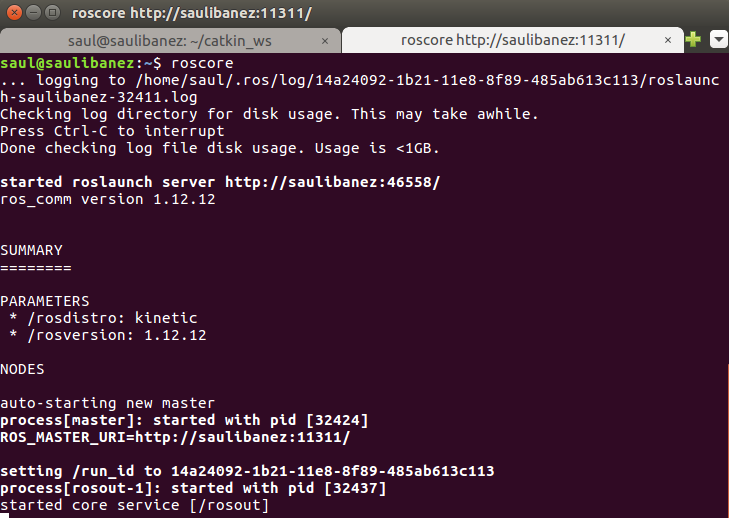
\includegraphics[width=11cm]{img/cap4/roscore}
  \end{center}
  \caption{Roscore}
  \label{fig:roscore}
\end{figure}
\newpage

Continuaremos lanzando el programa rosbridge.launch, que inciará el nodo de rosbridge para comunicarse con el robot, ejecutando el siguiente comando:

\begin{lstlisting}[caption=launch, label={lst:launch}]
	$ roslaunch openrov rosbridge.launch
\end{lstlisting}

\begin{figure} [hbtp]
  \begin{center}
    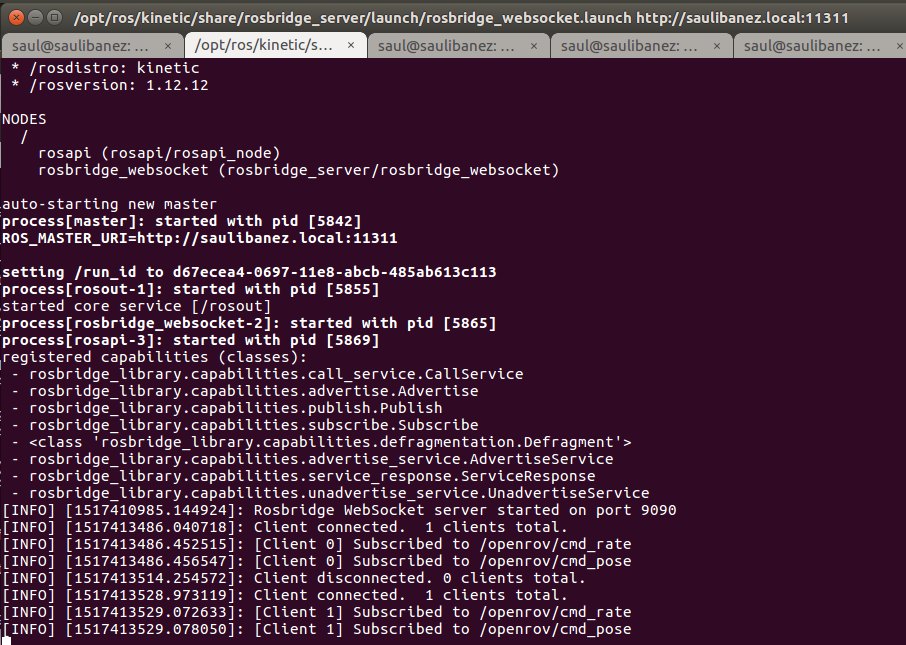
\includegraphics[width=11cm]{img/cap4/launch}
  \end{center}
  \caption{Launch}
  \label{fig:websocket.launch}
\end{figure}

También se comprobará en el terminal de OpenROV que la conexión se ha realizado.

\begin{figure} [hbtp]
  \begin{center}
    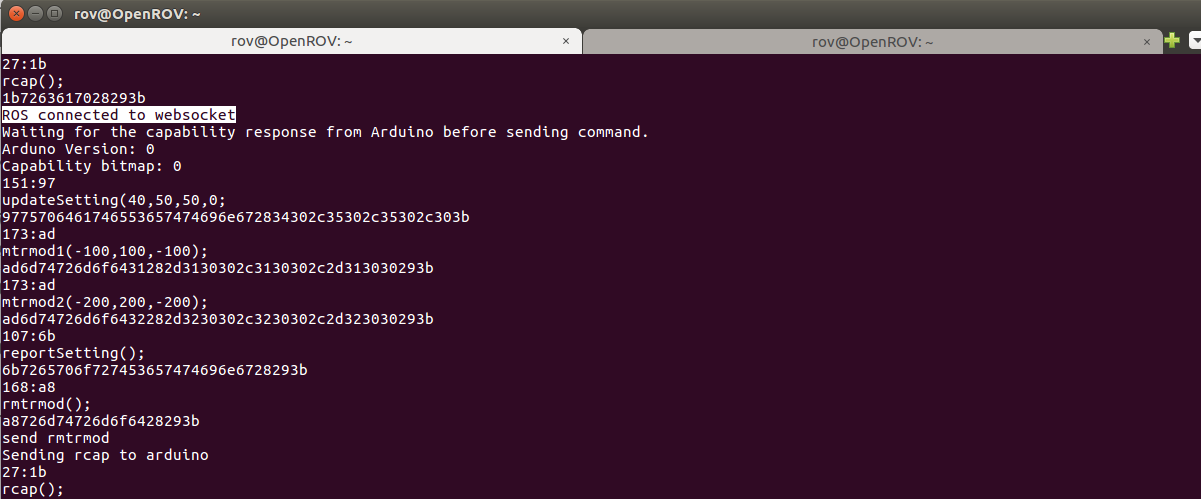
\includegraphics[width=14cm]{img/cap4/conexion_ROV}
  \end{center}
  \caption{Conexión en ROV}
  \label{fig:conect_rov}
\end{figure}

Para asegurarse de que todo esté funcionando, abriremos otra pestaña en el terminal e introduciremos:
\begin{lstlisting}[caption=rostopic list, label={lst:list}]
	$ rostopic list
\end{lstlisting}

Esto mostrará una lista de los temas que están siendo publicados por el ROV, así como algunos temas predeterminados.

\begin{figure} [hbtp]
  \begin{center}
    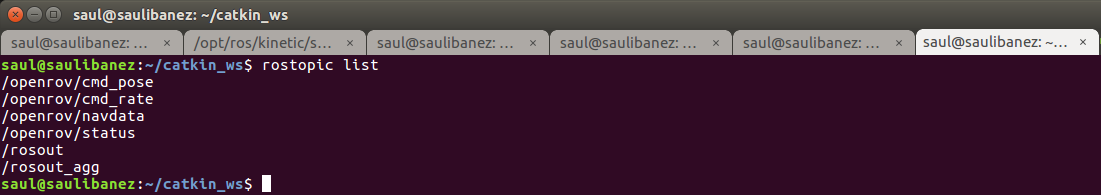
\includegraphics[width=14cm]{img/cap4/rostopic_list}
  \end{center}
  \caption{Rostopic list}
  \label{fig:rostopic_list}
\end{figure}

Para ver información sobre el nodo en particular, podremos ejecutar el comando: rostopic info.
\begin{lstlisting}[caption=rostopic info, label={lst:info}]
	$ rostopic info
\end{lstlisting}

\begin{figure} [hbtp]
  \begin{center}
    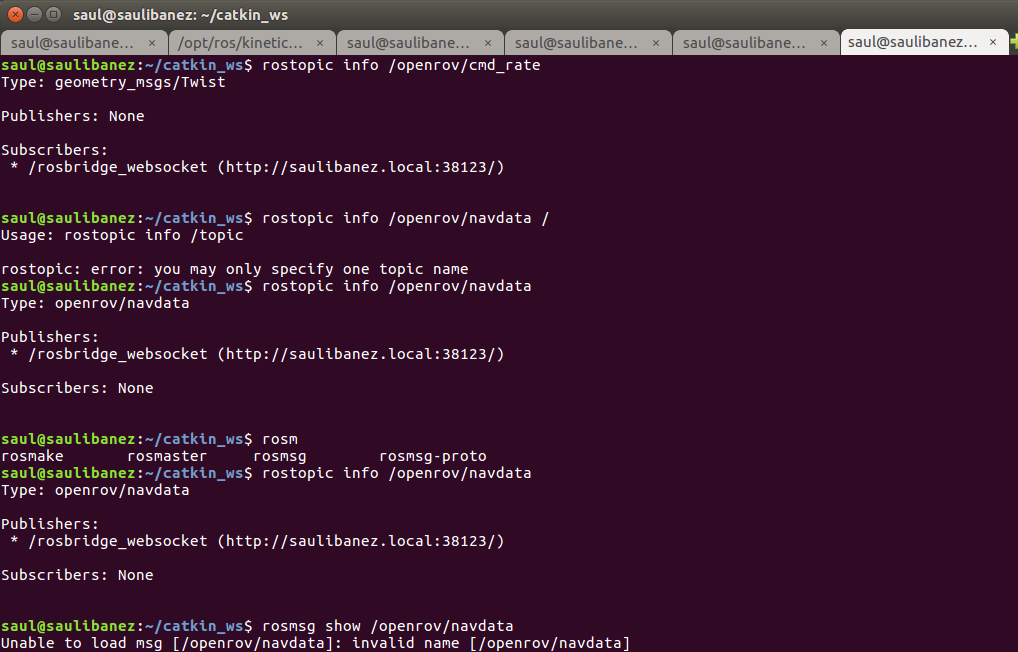
\includegraphics[width=12cm]{img/cap4/info1}
  \end{center}
  \caption{Rostopic info (1)}
  \label{fig:rostopic_info}
\end{figure}
\begin{figure} [hbtp]
  \begin{center}
    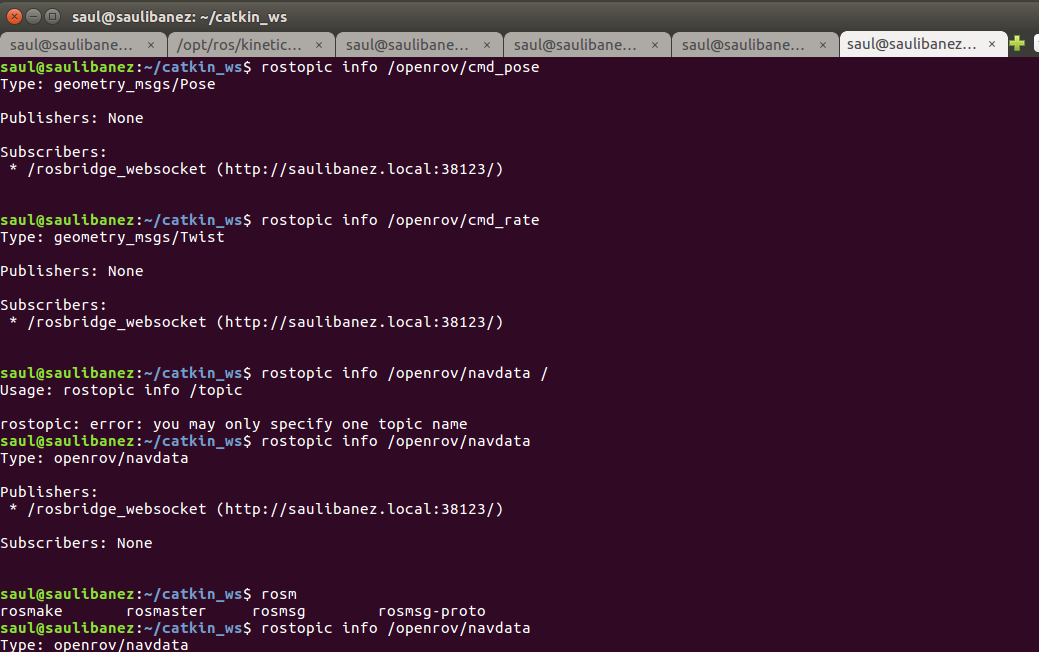
\includegraphics[width=12cm]{img/cap4/info2}
  \end{center}
  \caption{Rostopic info (2)}
  \label{fig:rostopic_info}
\end{figure}